\documentclass[12pt,a4paper]{report}

% ─── Packages ────────────────────────────────────────────────────────────────
\usepackage[T1]{fontenc}
\usepackage[utf8]{inputenc}

\usepackage[margin=1in,left=1.25in]{geometry}
\usepackage{setspace}
\usepackage{graphicx}
\usepackage{amsmath,amssymb,amsfonts}
\usepackage{array,tabularx,booktabs,longtable,multirow}
\usepackage{listings}
\usepackage{xcolor}
\usepackage{hyperref}
\usepackage{fancyhdr}
\usepackage{titlesec}
\usepackage{caption}
\usepackage{subcaption}
\usepackage{enumitem}
\usepackage{cite}
\usepackage{float}
\usepackage{afterpage}
\usepackage{mdframed}
\usepackage{tocloft}
\usepackage{algorithm}
\usepackage{algpseudocode}
\usepackage{tikz}
\usetikzlibrary{shapes.geometric,arrows.meta,positioning,fit,calc,matrix,chains}

% ─── Hyperref Setup ───────────────────────────────────────────────────────────
\hypersetup{
  colorlinks=true,
  linkcolor=black,
  citecolor=black,
  urlcolor=blue,
  pdftitle={UniZ: A Distributed University Administration Platform},
  pdfauthor={RGUKT ONG},
}

% ─── Page Style ───────────────────────────────────────────────────────────────
\pagestyle{fancy}
\fancyhf{}
\fancyhead[L]{\small UniZ: Distributed University Administration Platform}
\fancyhead[R]{\small\leftmark}
\fancyfoot[C]{\thepage}
\renewcommand{\headrulewidth}{0.4pt}

% ─── Code Listing Style ───────────────────────────────────────────────────────
\definecolor{codegray}{rgb}{0.5,0.5,0.5}
\definecolor{codeback}{rgb}{0.97,0.97,0.97}
\definecolor{codegreen}{rgb}{0,0.5,0}
\definecolor{codepurple}{rgb}{0.5,0,0.5}
\definecolor{codeblue}{rgb}{0,0,0.6}

\lstdefinestyle{jsonStyle}{
  backgroundcolor=\color{codeback},
  commentstyle=\color{codegreen},
  keywordstyle=\color{codeblue}\bfseries,
  stringstyle=\color{codepurple},
  basicstyle=\ttfamily\small,
  breakatwhitespace=false,
  breaklines=true,
  frame=single,
  rulecolor=\color{gray!40},
  numbers=left,
  numberstyle=\tiny\color{codegray},
  tabsize=2,
  showstringspaces=false,
  captionpos=b,
}

\lstset{style=jsonStyle}

% ─── Custom Commands ──────────────────────────────────────────────────────────
\newcommand{\api}[1]{\texttt{\small #1}}
\newcommand{\role}[1]{\texttt{#1}}
\newcommand{\field}[1]{\texttt{\textit{#1}}}
\newcommand{\code}[1]{\texttt{#1}}

\onehalfspacing

% ═══════════════════════════════════════════════════════════════════════════════
\begin{document}

% ─── Title Page ───────────────────────────────────────────────────────────────
\begin{titlepage}
\centering
\vspace*{0.5cm}
{\Large \textbf{RAJIV GANDHI UNIVERSITY OF KNOWLEDGE TECHNOLOGIES}}\\[0.3cm]
{\large ONGOLE, ANDHRA PRADESH -- 523001}\\[0.5cm]
\hrule height 1.5pt\vspace{0.3cm}\hrule height 0.5pt\vspace{0.8cm}
{\LARGE \textbf{A PROJECT REPORT}}\\[0.3cm]
{\large Submitted in partial fulfilment of the requirements for the}\\[0.2cm]
{\large \textbf{Bachelor of Technology in Computer Science and Engineering}}\\[1.2cm]
\begin{mdframed}[linewidth=1.5pt,innertopmargin=10pt,innerbottommargin=10pt]
\centering
{\Huge \textbf{UniZ}}\\[0.4cm]
{\Large A Distributed University Administration Platform with}\\[0.2cm]
{\Large Role-Based Access Control and Automated Approval Workflows}
\end{mdframed}
\vspace{1.2cm}
\begin{tabular}{ll}
\textbf{Platform:} & \url{https://uniz.rguktong.in} \\[4pt]
\textbf{API Base:} & \url{https://api.uniz.rguktong.in/api/v1} \\
\end{tabular}
\vspace{1.5cm}
{\large \textbf{Submitted by}}\\[0.4cm]
{\large RGUKT ONG Student Development Team}\\[0.8cm]
{\large \textbf{Under the Guidance of}}\\[0.3cm]
{\large Dr. [Faculty Guide Name]}\\[0.2cm]
{\normalsize Associate Professor, Department of Computer Science \& Engineering}\\[1.5cm]
{\normalsize\textbf{Department of Computer Science \& Engineering}\\
Rajiv Gandhi University of Knowledge Technologies\\
Ongole, Andhra Pradesh\\
Academic Year: 2025--2026}
\end{titlepage}

% ─── Certificate ──────────────────────────────────────────────────────────────
\newpage\thispagestyle{empty}
\begin{center}{\LARGE \textbf{CERTIFICATE}}\end{center}\vspace{0.8cm}
\noindent This is to certify that the project entitled \textbf{``UniZ: A Distributed University Administration Platform with Role-Based Access Control and Automated Approval Workflows''} is being submitted by the RGUKT ONG Student Development Team in partial fulfilment of the requirements for the degree of \textbf{Bachelor of Technology in Computer Science and Engineering} at Rajiv Gandhi University of Knowledge Technologies, Ongole. This work has been carried out under my supervision and is a bonafide record of independent work. To the best of my knowledge, the matter embodied in this report has not been submitted to any other university or institution.
\vspace{2.5cm}
\begin{tabular}{p{0.45\textwidth}p{0.45\textwidth}}
\makebox[0.45\textwidth]{\hrulefill} & \makebox[0.45\textwidth]{\hrulefill} \\
\textbf{Dr. [Faculty Guide]} & \textbf{Dr. [Head of Department]} \\
Associate Professor & Professor \& Head \\
Dept. of CSE, RGUKT ONG & Dept. of CSE, RGUKT ONG \\
\end{tabular}
\vspace{2cm}
\noindent \textbf{Place:} Ongole, Andhra Pradesh \quad \textbf{Date:} \today

% ─── Declaration ──────────────────────────────────────────────────────────────
\newpage\thispagestyle{empty}
\begin{center}{\LARGE \textbf{DECLARATION}}\end{center}\vspace{0.8cm}
\noindent We hereby declare that the project report entitled \textbf{``UniZ: A Distributed University Administration Platform with Role-Based Access Control and Automated Approval Workflows''} is a record of our original work carried out during the academic year 2025--2026. We further declare that: (i) the work contained herein has been carried out by us independently; (ii) the work has not been submitted to any other university for any degree; (iii) all sources are acknowledged; (iv) the architecture, API design, database schema, and security model described herein are the original intellectual contribution of the team.
\vspace{2cm}
\noindent \textbf{RGUKT ONG Student Development Team} \quad \textbf{Place:} Ongole \quad \textbf{Date:} \today

% ─── Acknowledgement ──────────────────────────────────────────────────────────
\newpage\thispagestyle{empty}
\begin{center}{\LARGE \textbf{ACKNOWLEDGEMENT}}\end{center}\vspace{0.8cm}
\noindent We express our sincere gratitude to our faculty guide, Dr. [Faculty Guide Name], for invaluable guidance and critical insights that shaped the architecture and methodology of this platform. We thank the Head of Department for providing the necessary laboratory infrastructure. We acknowledge the Director and Dean of RGUKT Ongole for administrative cooperation in defining operational requirements and validating the multi-level approval workflow. We are grateful to the hostel wardens, caretakers, Student Welfare Officers, security staff, and teaching faculty, whose domain expertise was instrumental in designing the role-based access control system, the outpass approval engine, and the academic data pipeline. Finally, we thank our fellow students who served as primary users and provided feedback during beta testing.

% ─── Abstract ─────────────────────────────────────────────────────────────────
\newpage\thispagestyle{empty}
\begin{center}{\LARGE \textbf{ABSTRACT}}\end{center}\vspace{0.8cm}

\noindent University administration in residential engineering institutions encompasses a heterogeneous set of operational concerns: academic record management, student campus mobility, hostel governance, gate security enforcement, and institutional communication. In the absence of integrated software systems, these concerns are managed through fragmented, paper-based workflows that introduce delays, data inconsistency, lack of audit trails, and significant administrative overhead.

\vspace{0.4cm}
\noindent This report presents \textbf{UniZ}, a distributed university administration platform purpose-built for Rajiv Gandhi University of Knowledge Technologies (RGUKT), Ongole. UniZ is architected as a Progressive Web Application (PWA) served at \url{https://uniz.rguktong.in}, backed by a RESTful API at \url{https://api.uniz.rguktong.in/api/v1}. The platform unifies five primary operational domains: student academic record management, outpass and outing request workflows, hostel administration, campus security gate operations, and institutional announcement management under a single, role-differentiated interface.

\vspace{0.4cm}
\noindent The platform implements a formal Role-Based Access Control (RBAC) model in which access permissions are determined by the function $\textsc{Access} = f(\text{role}, \text{resource}, \text{action})$. Nine distinct roles are modelled: \role{student}, \role{caretaker\_male}, \role{caretaker\_female}, \role{warden\_male}, \role{warden\_female}, \role{swo}, \role{dean}, \role{director}, \role{security}, \role{faculty}, and \role{webmaster}. Each role exposes a strictly bounded capability surface, enforced at both the API gateway and the database query layer.

\vspace{0.4cm}
\noindent The outpass approval engine implements a deterministic finite-state machine with six states: \texttt{caretaker} $\to$ \texttt{warden} $\to$ \texttt{swo} $\to$ \texttt{dean/director} $\to$ \texttt{approved} $\mid$ \texttt{rejected}. The system enforces the invariant $|R_{\text{active}}| \leq 1$, prohibiting concurrent active requests from a single student. Final authority roles (dean, director) possess an override capability that collapses the remaining approval chain to a terminal approved state.

\vspace{0.4cm}
\noindent Academic data management is designed for scale. Grade and attendance records are ingested through an asynchronous bulk-upload pipeline: Excel files are received via multipart HTTP, enqueued as background jobs, and processed in configurable batch sizes. Job state progresses through \texttt{queued} $\to$ \texttt{processing} $\to$ \texttt{completed} $\mid$ \texttt{failed}. Student-facing grade reads are served from a cache layer with sub-50\,ms p99 latency. Attendance percentage is computed server-side as $A = (\text{attended} / \text{total}) \times 100$.

\vspace{0.4cm}
\noindent Security is enforced through a JWT authentication lifecycle. All API requests require a Bearer token obtained at login. Tokens carry the authenticated role, enabling stateless RBAC enforcement at every endpoint. Password recovery is implemented via a time-bound, six-digit OTP. The campus gate security subsystem maintains a real-time presence model for every student, updated atomically on check-in and check-out events.

\vspace{0.6cm}
\noindent \textbf{Keywords:} Role-Based Access Control, Distributed Systems, REST API, Progressive Web Application, Approval Workflow, State Machine, Asynchronous Processing, University Administration, JWT Authentication.

\newpage\tableofcontents
\newpage\listoffigures
\newpage\listoftables

\newpage\pagenumbering{arabic}\setcounter{page}{1}

%%%% CHAPTER 1
\chapter{Introduction}

\section{Background and Motivation}

Residential engineering universities present a uniquely complex administrative environment. Unlike day-scholar institutions, a residential campus must simultaneously manage the academic lifecycle of enrolled students, the physical mobility of those students across campus boundaries, the logistics of hostel governance, and the enforcement of institutional security policies. In large-scale institutions such as Rajiv Gandhi University of Knowledge Technologies (RGUKT) with several hundred students per campus, these concerns have historically been addressed through paper-based workflows, verbal approvals, and disconnected spreadsheet records. The consequences of such fragmentation are well-documented: approval delays that stretch over days for processes that should complete in hours, data inconsistency between hostel registers and academic systems, absence of auditable logs, and a disproportionate administrative burden placed on faculty and staff.

The emergence of Progressive Web Applications (PWA) and cloud-hosted REST APIs has created an opportunity to consolidate these workflows into a unified, role-differentiated digital platform accessible from any device. The convergence of these technologies with mature software engineering practices in Role-Based Access Control (RBAC) and asynchronous processing pipelines makes it feasible to build production-grade administrative systems tailored to the specific operational model of residential universities.

\section{Problem Statement}

RGUKT Ongole operates with the following administrative pain points that motivated the development of UniZ:

\begin{enumerate}[label=(\arabic*)]
  \item \textbf{Manual outpass processing:} Student requests for campus exit are submitted on paper, passed manually through four approval levels (caretaker, warden, SWO, dean or director), and communicated to the security gate via physical documents. This pipeline takes 24--72 hours and offers no real-time status visibility to students or approvers.
  \item \textbf{Fragmented academic records:} Grade and attendance data are maintained in faculty-owned spreadsheets, communicated to administration via email, and consolidated manually. There is no single source of truth, and students have no real-time access to their academic standing.
  \item \textbf{No campus presence model:} The institution had no system to know, at any given moment, how many students were outside campus, when they left, and when they returned. Gate security relied on physical logbooks that were not searchable or auditable.
  \item \textbf{Absence of role-appropriate access control:} Staff accessed shared systems with no role-level restriction, creating risk of data exposure across administrative boundaries.
  \item \textbf{No institutional communication channel:} Campus announcements were distributed via WhatsApp groups or physical notice boards, with no guaranteed delivery or persistence.
\end{enumerate}

\section{Objectives}

The primary objectives of the UniZ project are:
\begin{enumerate}[label=(\arabic*)]
  \item Design and implement a formal RBAC model covering nine administrative roles with non-overlapping capability surfaces.
  \item Build a deterministic, multi-level outpass approval state machine with real-time status visibility and notification.
  \item Develop an asynchronous bulk academic data pipeline supporting grade and attendance upload for entire student cohorts.
  \item Implement a real-time campus presence model maintained by security staff at entry and exit gates.
  \item Deploy the platform as a cross-platform PWA accessible on any device without application store dependency.
  \item Secure all data access through JWT-based authentication with role-embedded claims and OTP-based password recovery.
\end{enumerate}

\section{Scope}

The functional scope of UniZ includes: (1) \textbf{Student Module} -- academic record viewing, outpass and outing request submission, request history, and profile management; (2) \textbf{Admin Module} -- role-differentiated approval dashboards, student search, bulk student onboarding, banner management, and academic publishing; (3) \textbf{Faculty Module} -- grade and attendance upload via Excel templates, background job monitoring; (4) \textbf{Security Module} -- real-time approved-pass verification, gate check-in and check-out logging, campus presence monitoring; (5) \textbf{System Module} -- public health check endpoint, JWT authentication, OTP-based password recovery.

\section{Report Organisation}

Chapter~2 provides a system overview. Chapter~3 formalises the RBAC model. Chapters~4--6 detail the student, admin, and faculty modules. Chapter~7 presents the complete API specification. Chapter~8 describes the system architecture. Chapter~9 covers database design. Chapter~10 analyses security. Chapter~11 presents the approval engine. Chapter~12 addresses performance. Chapter~13 covers error handling. Chapter~14 offers discussion. Chapter~15 concludes. References and appendices follow.

%%%% CHAPTER 2
\chapter{System Overview}

\section{Platform Identity and Deployment}

UniZ (University Intelligence Zone) is an enterprise-grade, web-first university administration platform deployed at RGUKT Ongole. The platform is publicly accessible at \url{https://uniz.rguktong.in} and exposes its programmatic interface via a versioned REST API at \url{https://api.uniz.rguktong.in/api/v1}. The platform is structured as a client-server system with strict separation of concerns: all business logic, data persistence, access control enforcement, and external service integration reside on the server; the client is a thin, stateless PWA responsible solely for rendering and user interaction.

\section{Technology Stack}

\subsection{Client Layer}
The frontend is implemented as a Progressive Web Application, enabling installation on iOS (via Safari's Add to Home Screen mechanism), Android (via Chrome install banner), and desktop operating systems through Chromium-based browsers. Installation delivers a full-screen, app-like experience without requiring app store distribution. The PWA service worker enables offline caching of static assets, ensuring the interface remains accessible during intermittent network conditions.

\subsection{API Layer}
The backend exposes a RESTful HTTP API using JSON as its sole wire format. All endpoints are versioned under the \api{/api/v1/} prefix. The API is stateless: every request carries its own authentication token, and no server-side session state is maintained between requests. This design enables horizontal scaling of API server instances behind a load balancer without session affinity requirements.

\subsection{Authentication}
Authentication is implemented via JSON Web Tokens (JWT). Upon successful credential verification, the server issues a signed token containing the authenticated user's role claim. This token is presented in the \code{Authorization: Bearer <token>} header of every subsequent request. The server validates the token's signature and role claim at the API gateway, prior to any route handler execution.

\subsection{Background Processing}
Bulk academic data operations (grade and attendance uploads, result publishing via email) are executed asynchronously through a background job queue. File ingestion via multipart HTTP is decoupled from record processing: the upload endpoint acknowledges receipt immediately, assigns a job identifier, and delegates processing to a worker process. Clients poll a progress endpoint to track completion.

\section{Architectural Layers}

The system follows a layered architecture comprising: (1) Presentation Layer -- PWA frontend over HTTPS; (2) API Gateway Layer -- JWT validation, RBAC enforcement, rate limiting; (3) Service Layer -- domain business logic; (4) Data Access Layer -- parameterised database queries; (5) Persistence Layer -- relational database plus cache layer; (6) Async Worker Layer -- background job executor; (7) External Service Layer -- institutional email (SMTP).

Figure~\ref{fig:arch} illustrates the high-level system architecture.

\begin{figure}[H]
\centering
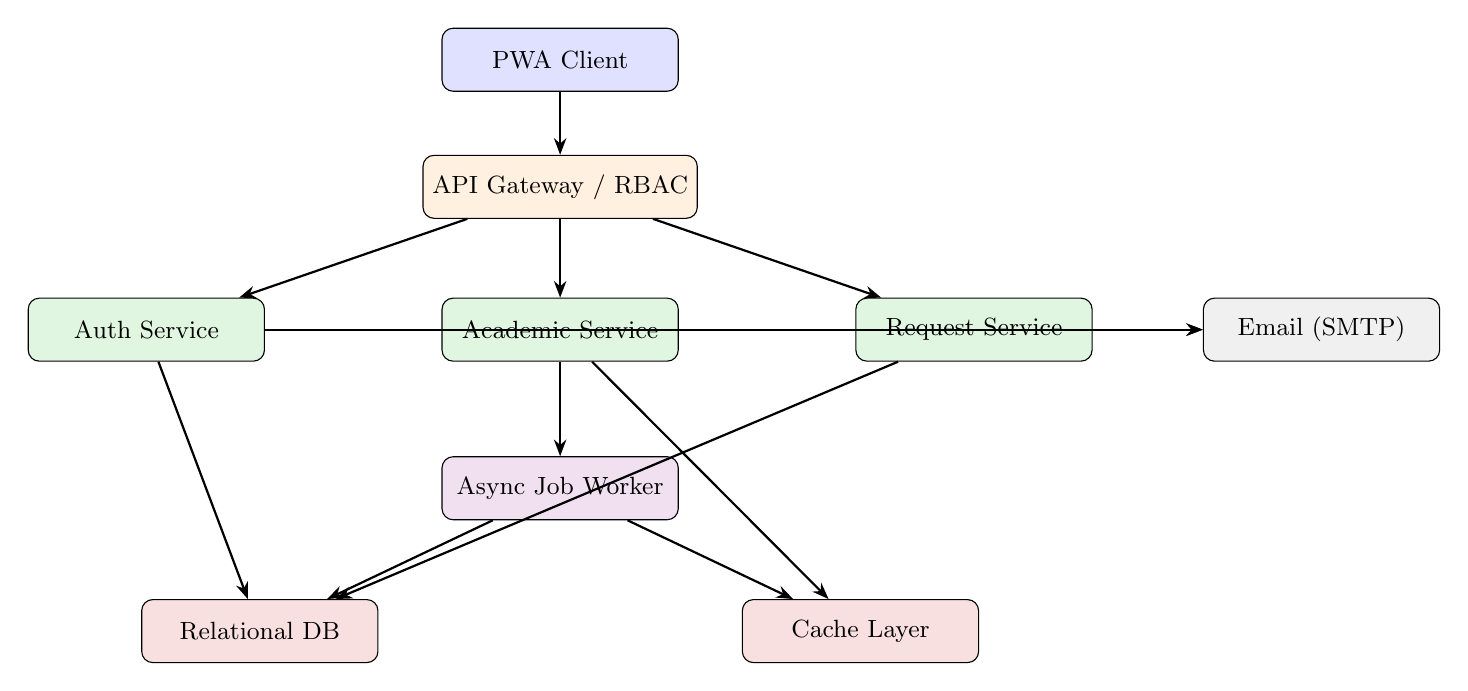
\begin{tikzpicture}[
  font=\small,
  node distance=0.8cm and 1.5cm,
  box/.style={draw,rounded corners=4pt,fill=#1!12,minimum width=3cm,minimum height=0.8cm,align=center,font=\small},
  arrow/.style={-{Stealth[length=6pt]},thick},
]
\node[box=blue] (pwa)    {PWA Client};
\node[box=orange, below=of pwa] (gw)  {API Gateway / RBAC};
\node[box=green!70!black, below left=1cm and 2cm of gw]   (auth)  {Auth Service};
\node[box=green!70!black, below=1cm of gw]                (acad)  {Academic Service};
\node[box=green!70!black, below right=1cm and 2cm of gw]  (req)   {Request Service};
\node[box=violet, below=1.2cm of acad]  (worker) {Async Job Worker};
\node[box=red!80!black, below left=1cm and 0.8cm of worker]  (db)    {Relational DB};
\node[box=red!80!black, below right=1cm and 0.8cm of worker] (cache) {Cache Layer};
\node[box=gray, right=1.4cm of req]     (mail)  {Email (SMTP)};
\draw[arrow] (pwa) -- (gw);
\draw[arrow] (gw) -- (auth);
\draw[arrow] (gw) -- (acad);
\draw[arrow] (gw) -- (req);
\draw[arrow] (acad) -- (worker);
\draw[arrow] (worker) -- (db);
\draw[arrow] (worker) -- (cache);
\draw[arrow] (auth) -- (db);
\draw[arrow] (req) -- (db);
\draw[arrow] (acad) -- (cache);
\draw[arrow] (req) -- (mail);
\draw[arrow] (auth) -- (mail);
\end{tikzpicture}
\caption{UniZ high-level system architecture}
\label{fig:arch}
\end{figure}

\section{System Health Monitoring}

The system exposes a public, unauthenticated health check endpoint at \api{GET /system/health} that returns the operational status and measured latency of each internal service. Listing~\ref{lst:health} shows a representative response.

\begin{lstlisting}[caption={System health check response},label={lst:health}]
{
  "success": true,
  "services": [
    { "name": "Auth Service", "status": "UP", "latency": "120ms" },
    { "name": "Mail Service", "status": "UP", "latency": "45ms"  }
  ]
}
\end{lstlisting}

%%%% CHAPTER 3
\chapter{User Roles and the RBAC Model}

\section{Formal RBAC Definition}

UniZ implements a flat, non-hierarchical Role-Based Access Control model in which every access decision is determined by:

\begin{equation}
  \textsc{Access}(u, r, a) = \begin{cases} \text{Permit} & \text{if } \exists\, \rho \in \text{Roles}(u) \text{ such that } (r, a) \in P(\rho) \\ \text{Deny} & \text{otherwise} \end{cases}
  \label{eq:rbac}
\end{equation}

where $u$ is the authenticated user, $r$ is the requested resource, $a$ is the requested action, $\text{Roles}(u)$ is the singleton role assigned to $u$ at account creation, and $P(\rho)$ is the permission set of role $\rho$. A user's role is immutable after assignment; there is no runtime role-switching mechanism.

\section{Role Catalogue}

Table~\ref{tab:roles} presents the complete role catalogue.

\begin{table}[H]
\centering
\caption{UniZ role catalogue}
\label{tab:roles}
\renewcommand{\arraystretch}{1.3}
\begin{tabularx}{\textwidth}{llX}
\toprule
\textbf{Role} & \textbf{Username Pattern} & \textbf{Primary Domain} \\
\midrule
\code{student}           & \code{O210008}             & Academic records, mobility requests \\
\code{caretaker\_male}   & \code{caretaker\_male}     & First-level outpass approval (male hostel) \\
\code{caretaker\_female} & \code{caretaker\_female}   & First-level outpass approval (female hostel) \\
\code{warden\_male}      & \code{warden\_male}        & Second-level outpass approval (male hostel) \\
\code{warden\_female}    & \code{warden\_female}      & Second-level outpass approval (female hostel) \\
\code{swo}               & \code{swo}                 & Third-level outpass approval \\
\code{dean}              & \code{dean\_cse}           & Final approval, academic oversight \\
\code{director}          & \code{director}            & Super authority, global override \\
\code{security}          & \code{security\_admin}     & Gate check-in/check-out \\
\code{faculty}           & \code{faculty\_<id>}       & Grade and attendance upload \\
\code{webmaster}         & \code{webmaster}           & Banner management, system health \\
\bottomrule
\end{tabularx}
\end{table}

\section{Permission Matrix}

Table~\ref{tab:perm} maps roles to actions across primary resource domains.

\begin{table}[H]
\centering
\caption{Role-resource permission matrix ($\checkmark$ = full; $\circ$ = read-only; $-$ = none)}
\label{tab:perm}
\renewcommand{\arraystretch}{1.2}
\small
\begin{tabular}{lccccccc}
\toprule
\textbf{Resource} & \textbf{Student} & \textbf{Caretaker/Warden} & \textbf{SWO} & \textbf{Dean} & \textbf{Director} & \textbf{Security} & \textbf{Faculty} \\
\midrule
Own grades (read)       & $\checkmark$ & $-$ & $-$ & $\circ$ & $\circ$ & $-$ & $\circ$ \\
Batch grades (read)     & $-$ & $-$ & $-$ & $\checkmark$ & $\checkmark$ & $-$ & $\circ$ \\
Grade write             & $-$ & $-$ & $-$ & $\checkmark$ & $\checkmark$ & $-$ & $\checkmark$ \\
Attendance (read)       & $\checkmark$ & $-$ & $-$ & $\circ$ & $\circ$ & $-$ & $\checkmark$ \\
Attendance write        & $-$ & $-$ & $-$ & $-$ & $-$ & $-$ & $\checkmark$ \\
Submit outpass          & $\checkmark$ & $-$ & $-$ & $-$ & $-$ & $-$ & $-$ \\
View all outpasses      & $-$ & $\checkmark$ & $\checkmark$ & $\checkmark$ & $\checkmark$ & $\checkmark$ & $-$ \\
Approve outpass         & $-$ & $\checkmark$ & $\checkmark$ & $\checkmark$ & $\checkmark$ & $-$ & $-$ \\
Gate check-in/out       & $-$ & $-$ & $-$ & $-$ & $\checkmark$ & $\checkmark$ & $-$ \\
Status override         & $-$ & $-$ & $-$ & $-$ & $\checkmark$ & $-$ & $-$ \\
Publish results (email) & $-$ & $-$ & $-$ & $-$ & $\checkmark$ & $-$ & $-$ \\
\bottomrule
\end{tabular}
\end{table}

\section{Gender-Partitioned Roles}

Caretaker and warden roles are partitioned by student gender. Each partitioned role can access only the request queue for students of the corresponding gender, determined by the \field{studentGender} field on each request record. This ensures hostel staff operate within their designated hostel only, reducing cross-hostel data exposure.

\section{Role Assignment and Immutability}

Roles are assigned at account creation by a system administrator and persisted as an attribute of the user record. No API endpoint exists to change a user's own role; role modification requires direct database access by a system administrator. This design eliminates privilege escalation attacks through the application layer.

%%%% CHAPTER 4
\chapter{Student Module}

\section{Overview}

The student module provides enrolled students with access to academic records, campus mobility request management, and personal profile information. All student-facing functionality is gated behind authentication using the university roll number (e.g., \code{O210008}) as the username.

\section{Academic Record Access}

\subsection{Grade Records}

Students access grade records via \api{GET /academics/grades}. The response includes all grade records across all semesters, each carrying the subject code, name, credit hours, letter grade, and semester identifier. Grade data is served from the cache layer, yielding sub-50\,ms response times. The \field{source} field indicates whether the record was served from \code{"cache"} or \code{"db"}, providing data freshness transparency.

\subsection{Attendance Records}

Attendance is fetched via \api{GET /academics/attendance}, returning per-subject data with raw counts (\field{attendedClasses}, \field{totalClasses}). The attendance percentage $A$ for a given subject is:

\begin{equation}
  A = \frac{\text{attendedClasses}}{\text{totalClasses}} \times 100
  \label{eq:attendance}
\end{equation}

Regulatory policy at RGUKT mandates minimum attendance of 75\% for examination eligibility. The client renders a warning when $A < 75$ for any subject.

\section{Outpass and Outing Requests}

\subsection{Request Type Distinction}

UniZ models two campus exit request types. \textbf{Outpass} is a multi-day leave request for home visits, medical treatment, or family events, specifying \field{fromDay} and \field{toDay}, requiring traversal of the full four-level approval chain. \textbf{Outing} is a same-day, short-duration exit for brief errands, specifying \field{fromTime} and \field{toTime} on the same calendar day, following a lighter approval path.

\subsection{Outpass Submission}

A student submits an outpass via \api{POST /requests/outpass}. The server enforces the active-request constraint:

\begin{equation}
  |R_{\text{active}}(s)| \leq 1 \quad \forall\, s \in \text{Students}
  \label{eq:constraint}
\end{equation}

where $R_{\text{active}}(s)$ is the set of non-terminal requests for student $s$. A student with a pending request must await its resolution before submitting a new one.

\subsection{Outing Submission}

An outing is submitted via \api{POST /requests/outing} with reason, \field{fromTime}, and \field{toTime}. Both times must fall on the same calendar day; the server returns \code{400 Bad Request} if they span midnight.

\subsection{Rate Limiting}

Both submission endpoints are rate-limited to prevent abuse. Requests exceeding the threshold receive \code{429 Too Many Requests}.

\subsection{Request History}

Students retrieve their full request history via \api{GET /requests/history}, which returns all past outpass and outing requests sorted newest-first with pagination.

\section{Profile Management}

Student profiles carry: full name (uppercase, per university records), roll number, branch, academic year (E1--E4), registered institutional email, and current campus presence status (\field{is\_in\_campus}). Students may update personal contact details through the profile management endpoint.

%%%% CHAPTER 5
\chapter{Admin Module}

\section{Overview}

The admin module serves caretaker, warden, SWO, dean, director, security, and webmaster roles. All authenticate via \api{POST /auth/login}; the server determines the capability surface from the role embedded in the issued JWT.

\section{Approvals Subsystem}

\subsection{Approval Queue Architecture}

The approvals subsystem maintains a shared request collection. Each record carries \field{currentLevel} indicating the approval role that must act next. The \api{GET /requests/outpass/all} endpoint returns all records without server-side role filtering; client-side filtering is applied by role. This design decouples the approval view from the data model, allowing authorised roles to inspect records for audit purposes.

\subsection{Approve Action}

An approver calls \api{POST /requests/:id/approve}. The server validates that the caller's role is consistent with the request's \field{currentLevel}, then executes:

\begin{equation}
  \delta(\text{currentLevel}, \text{approve}) = \text{next}(\text{currentLevel})
  \label{eq:approve}
\end{equation}

where next maps: \code{caretaker} $\to$ \code{warden} $\to$ \code{swo} $\to$ \code{dean/director} $\to$ \code{approved}.

\subsection{Reject Action}

Rejection via \api{POST /requests/:id/reject} terminates the request in the rejected terminal state. A comment is mandatory; the server returns \code{400} if absent. The student receives an immediate notification containing the rejection reason.

\subsection{Final Authority Override}

Dean and director approval collapses the chain to the approved state regardless of current level:

\begin{equation}
  \delta(\ell, \text{approve}) = \texttt{approved} \quad \text{if } \text{role}(u) \in \{\texttt{dean}, \texttt{director}\}
  \label{eq:override}
\end{equation}

Upon reaching approved, the student is notified and the record becomes visible to security for gate verification.

\subsection{Request Expiry}

A background scheduled task identifies requests whose \field{fromDay} has elapsed while non-terminal. Such requests are transitioned to an expired soft state: \field{isExpired} is set to \code{true}. Expired records are retained for audit but cannot receive further approval actions.

\section{Student Search and Profiling}

Dean and director roles have access to \api{POST /profile/student/search} with flexible filter criteria: username, name fragment, branch, year, campus presence status, and pagination. The director has unrestricted search scope across all students.

\section{Academic Management}

\subsection{Batch Grade Viewing}

\api{GET /academics/grades/batch} accepts branch, year, semesterId, and optional \field{failedOnly} boolean. The response summary includes aggregate counts for academic risk assessment.

\subsection{Bulk Grade Correction}

\api{PUT /academics/grades/bulk-update} accepts an array of correction objects, each with student ID, subject UUID, semester ID, and new grade. Invalid subject IDs are silently skipped.

\subsection{Result Publication}

\api{POST /academics/grades/publish-email}, restricted to the director, triggers a background bulk-email job dispatching grade report cards to all students for the specified semester. Progress is monitored via \api{GET /academics/grades/publish/progress}.

\subsection{Student Bulk Onboarding}

New cohorts are onboarded by downloading the student template (\api{GET /admin/student/template}), populating it with roll numbers, full names, and institutional emails, then uploading via \api{POST /admin/student/upload}. Processing is asynchronous, returning a jobId for progress polling.

\section{Banner Management}

Banners are created in draft state (\field{isPublished}: \code{false}) and explicitly published via \api{POST /profile/admin/banners/:id/publish}. Published banners appear to all authenticated users. Only the webmaster can create and publish; dean and director have read-only visibility.

\section{Security Portal}

\subsection{Dashboard Metrics}

\api{GET /requests/security/summary} returns total students outside campus, today's check-in count, and today's check-out count. The dashboard polls this endpoint every 30 seconds when active.

\subsection{Gate Check-Out}

The security officer verifies \field{isApproved}: \code{true} on the student's request record, cross-checks the date window, and calls \api{POST /requests/:id/checkout}, setting \field{is\_in\_campus} to \code{false} atomically.

\subsection{Gate Check-In}

\api{POST /requests/:id/checkin} sets \field{is\_in\_campus} to \code{true} and records the entry timestamp.

\subsection{Manual Status Correction}

\api{PUT /profile/student/status} allows director or security to directly set campus presence, intended exclusively for correcting data errors from system failures.

%%%% CHAPTER 6
\chapter{Faculty Module}

\section{Overview}

The faculty module serves teaching staff responsible for submitting grade and attendance data. Faculty interact via a template-download, fill-and-upload workflow optimised for bulk data entry, supplemented by single-record endpoints for individual corrections.

\section{Grade Management}

\subsection{Template-Based Bulk Upload}

The canonical grade submission workflow is:
\begin{enumerate}[label=(\arabic*)]
  \item \textbf{Download template:} \api{GET /academics/grades/template} with branch, year, semester, subjectCode. Returns a pre-populated \code{.xlsx} file.
  \item \textbf{Populate:} Faculty fill the grade column. Valid values are letter grades (\code{EX}, \code{A}, \code{B}, \code{C}, \code{D}, \code{F}) or numeric grade point values.
  \item \textbf{Upload:} \api{POST /academics/grades/upload} with the completed file. Server acknowledges immediately, returning a \field{jobId}.
  \item \textbf{Monitor:} Poll \api{GET /academics/grades/upload/progress} to track background processing.
\end{enumerate}

\subsection{Asynchronous Processing Pipeline}

The upload pipeline is:
\begin{equation}
  \text{File} \xrightarrow{\text{HTTP}} \text{Queue} \xrightarrow{\text{Worker}} \text{Parse \& Validate} \xrightarrow{\text{DB write}} \text{Cache invalidate}
\end{equation}

Validation rules: roll number must match an existing student; subject code must match a registered subject; grade value must conform to the accepted type union. Records failing validation are logged to a per-job error collection without aborting the job.

\subsection{Job State Machine}

Upload jobs transition through four states as shown in Figure~\ref{fig:jobstate}.

\begin{figure}[H]
\centering
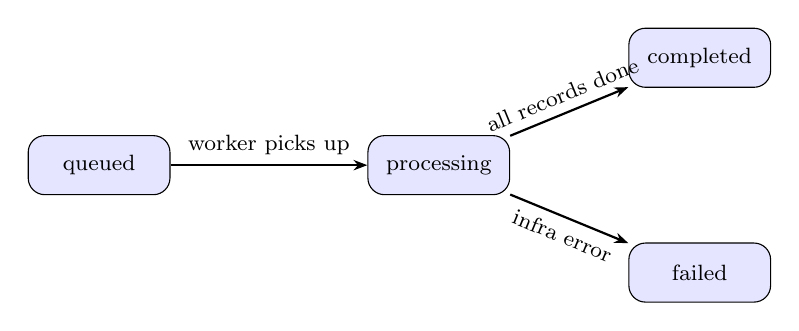
\begin{tikzpicture}[
  font=\small,
  node distance=2.5cm,
  state/.style={draw,rounded corners=6pt,fill=blue!10,minimum width=1.8cm,minimum height=0.75cm,align=center,font=\footnotesize},
  arrow/.style={-{Stealth[length=5pt]},thick},
]
\node[state] (q) {queued};
\node[state, right=of q] (p) {processing};
\node[state, above right=0.6cm and 1.5cm of p] (c) {completed};
\node[state, below right=0.6cm and 1.5cm of p] (f) {failed};
\draw[arrow] (q) -- node[font=\footnotesize,above]{worker picks up} (p);
\draw[arrow] (p) -- node[font=\footnotesize,above,sloped]{all records done} (c);
\draw[arrow] (p) -- node[font=\footnotesize,below,sloped]{infra error} (f);
\end{tikzpicture}
\caption{Upload job state machine}
\label{fig:jobstate}
\end{figure}

\subsection{Single-Record Grade Add}

For individual grade entries, faculty call \api{POST /academics/grades/add} synchronously with student ID, subject UUID, semester ID, and grade value.

\section{Attendance Management}

Attendance submission mirrors the grade workflow. Faculty download a template via \api{GET /academics/attendance/template}, populate the \field{attended} boolean column, and upload via \api{POST /academics/attendance/upload}. Single-record attendance is added via \api{POST /academics/attendance/add} with optional date parameter (defaulting to today). Compiled reports are downloaded via \api{GET /academics/attendance/download/:semesterId}.

%%%% CHAPTER 7
\chapter{API Design}

\section{Design Principles}

The UniZ REST API adheres to: (1) \textbf{Versioning} via \api{/api/v1/} prefix; (2) \textbf{Statelessness} -- all authentication context in JWT; (3) \textbf{Consistent response envelope} -- top-level \field{success} boolean; (4) \textbf{ISO~8601 timestamps} in UTC; (5) \textbf{HTTP verb semantics} -- GET for reads, POST for creates/actions, PUT for bulk updates.

\section{Authentication Endpoints}

\subsection{POST /auth/login}

\textbf{Role access:} All. \textbf{Request:}
\begin{lstlisting}[caption={Login request},label={lst:login}]
{ "username": "O210008", "password": "your_password" }
\end{lstlisting}
\textbf{Response (200):}
\begin{lstlisting}[caption={Login response},label={lst:loginres}]
{ "success": true, "token": "eyJ...", "role": "student", "username": "O210008" }
\end{lstlisting}
\textbf{Errors:} 400 (missing fields), 401 (invalid credentials).

\subsection{POST /auth/otp}

\textbf{Role access:} All (unauthenticated). Sends a six-digit OTP to registered email. OTP is time-bound and single-use. \textbf{Request:} \code{\{"username": "O210008"\}}. \textbf{Response:} \code{\{"success": true, "message": "OTP sent to registered email"\}}.

\section{Grade Endpoints}

\subsection{GET /academics/grades}
\textbf{Role:} Student. \textbf{Cache:} Sub-50\,ms from cache layer. \textbf{Response:}
\begin{lstlisting}[caption={Student grades},label={lst:grades}]
{
  "success": true, "source": "cache",
  "grades": [
    { "id": "abc-123", "grade": "EX", "semesterId": "E3S1",
      "subject": { "code": "CS3101", "name": "Operating Systems", "credits": 4 } }
  ]
}
\end{lstlisting}

\subsection{GET /academics/grades/batch}
\textbf{Role:} Webmaster, Dean, Director. \textbf{Query params:} branch, year, semesterId, failedOnly.
\begin{lstlisting}[caption={Batch grades response},label={lst:batchgrades}]
{
  "success": true,
  "summary": { "totalStudents": 3, "totalRecords": 7, "failedRecords": 2,
               "timestamp": "2026-02-01T10:00:00Z" },
  "students": [
    { "studentId": "O210139", "name": "DAMARLA SEETHA RAM PRAVEEN",
      "branch": "CSE", "year": "E2",
      "records": [
        { "subjectCode": "E2-SEM-1-CSE-3",
          "subjectName": "Design & Analysis of Algorithms",
          "grade": 0, "credits": 4, "semesterId": "SEM-1" }
      ] }
  ]
}
\end{lstlisting}

\subsection{POST /academics/grades/add}
\textbf{Role:} Faculty, Admin. \textbf{Body:} studentId, subjectId (UUID), semesterId, grade. \textbf{Response:} \code{\{"success": true, "message": "Grade added successfully"\}}.

\subsection{PUT /academics/grades/bulk-update}
\textbf{Role:} Webmaster, Dean. \textbf{Body:} updates array of \{studentId, subjectId, semesterId, grade\}. Invalid subject IDs silently skipped. \textbf{Response:} includes \field{updated} count.

\subsection{GET /academics/grades/template}
\textbf{Role:} Faculty, Admin. Returns binary \code{.xlsx} pre-populated with student IDs. \textbf{Query:} branch, year, semester, subjectCode.

\subsection{POST /academics/grades/upload}
\textbf{Role:} Faculty, Admin. \textbf{Content-Type:} multipart/form-data. \textbf{Response:}
\begin{lstlisting}[caption={Upload initiated},label={lst:uploadstart}]
{ "success": true, "message": "Upload started", "jobId": "job-abc-123" }
\end{lstlisting}

\subsection{GET /academics/grades/upload/progress}
\textbf{Role:} Faculty, Admin.
\begin{lstlisting}[caption={Upload progress},label={lst:progress}]
{
  "success": true,
  "progress": { "status": "processing", "percent": 45,
                "processed": 150, "total": 330 }
}
\end{lstlisting}
Status values: \code{queued}, \code{processing}, \code{completed}, \code{failed}.

\subsection{POST /academics/grades/publish-email}
\textbf{Role:} Director only. \textbf{Body:} \code{\{"semesterId": "SEM-1"\}}. Triggers irreversible bulk email. Poll \api{GET /academics/grades/publish/progress} for status.

\section{Attendance Endpoints}

\subsection{GET /academics/attendance}
\textbf{Role:} Student. Returns per-subject records with attendedClasses, totalClasses, and subject object.

\subsection{POST /academics/attendance/add}
\textbf{Role:} Faculty. \textbf{Body:} studentId, subjectId, semesterId, attended (boolean), date (optional, defaults to today).

\subsection{GET /academics/attendance/template} \textbf{Role:} Faculty, Admin. Returns binary \code{.xlsx} template.

\subsection{POST /academics/attendance/upload} \textbf{Role:} Faculty, Admin. Returns jobId.

\subsection{GET /academics/attendance/upload/progress} \textbf{Role:} Faculty, Admin. Identical structure to grade upload progress.

\section{Outpass Endpoints}

\subsection{POST /requests/outpass}
\textbf{Role:} Student.
\begin{lstlisting}[caption={Outpass submission},label={lst:outpassreq}]
{
  "reason":        "Emergency home visit",
  "fromDay":       "2026-02-10T09:00:00Z",
  "toDay":         "2026-02-15T18:00:00Z",
  "studentGender": "M"
}
\end{lstlisting}
\textbf{Constraints:} reason required; fromDay must be future; toDay after fromDay; no active request ($|R_{\text{active}}| = 0$). \textbf{Errors:} 400 (invalid fields), 401 (no token), 409 (active request exists), 429 (rate limited).
\begin{lstlisting}[caption={Outpass response},label={lst:outpassres}]
{
  "success": true,
  "data": { "id": "req-789", "currentLevel": "caretaker",
            "isApproved": false, "createdAt": "2026-01-31T10:00:00Z" }
}
\end{lstlisting}

\subsection{GET /requests/outpass/all}
\textbf{Role:} Caretaker, Warden, Dean, Director, Security. Returns all records; client filters by currentLevel.

\subsection{GET /requests/history} \textbf{Role:} Student. Paginated history with type, status, reason, requested\_time.

\subsection{GET /requests/outside} \textbf{Role:} Admin, Security, Director. Students currently outside campus with active approved outpass.

\section{Outing Endpoints}

\subsection{POST /requests/outing}
\textbf{Role:} Student.
\begin{lstlisting}[caption={Outing submission},label={lst:outingreq}]
{ "reason": "Buying groceries",
  "fromTime": "2026-02-10T17:00:00Z", "toTime": "2026-02-10T20:00:00Z" }
\end{lstlisting}
\textbf{Constraint:} fromTime and toTime must be same calendar day.

\subsection{GET /requests/outing/all} \textbf{Role:} Security, Director, Admin. Used for gate verification of same-day exits.

\section{Approval Action Endpoints}

\subsection{POST /requests/:id/approve}
\textbf{Role:} Caretaker, Warden, SWO, Dean, Director. Optional comment. Advances currentLevel. If caller is Dean/Director, sets isApproved: true immediately.

\subsection{POST /requests/:id/reject}
\textbf{Role:} Caretaker, Warden, SWO, Dean, Director. Comment required. Sets isRejected: true; notifies student.

\subsection{POST /requests/:id/forward} Semantic alias for approve. Same backend effect.

\section{Gate Control and Security Endpoints}

\subsection{POST /requests/:id/checkout} \textbf{Role:} Security, Director. Sets is\_in\_campus: false; records exit time. \textbf{Response:} \code{\{"success": true, "msg": "Checked-Out"\}}.

\subsection{POST /requests/:id/checkin} \textbf{Role:} Security, Director. Sets is\_in\_campus: true. \textbf{Response:} \code{\{"success": true, "msg": "Checked-In"\}}.

\subsection{GET /requests/security/summary}
\begin{lstlisting}[caption={Security summary},label={lst:secsummary}]
{ "success": true, "summary": { "totalOutside": 14, "todayCheckins": 8, "todayCheckouts": 22 } }
\end{lstlisting}

%%%% CHAPTER 8
\chapter{System Architecture}

\section{Architectural Style}

UniZ adopts a service-oriented, layered architectural style. Concerns are separated across well-defined horizontal layers, enabling independent scaling, testability, and maintainability.

\section{Progressive Web Application}

The client is a Progressive Web Application conforming to the PWA specification. Key properties include: (1) \textbf{Service Worker} -- intercepts network requests, enabling static asset caching and offline fallback; (2) \textbf{Web App Manifest} -- provides metadata for home screen installation; (3) \textbf{HTTPS-only} -- required by the PWA spec, aligning with the security posture. Installation mechanics differ by platform: Android Chrome presents an install banner; iOS Safari requires the Add to Home Screen action; desktop uses the browser install icon.

\section{API Server Architecture}

The API server is stateless and fronted by an API gateway responsible for: (1) JWT validation; (2) RBAC enforcement; (3) rate limiting; (4) request routing. Statelessness enables horizontal scaling without session affinity.

\section{Data Flow Diagram}

Figure~\ref{fig:dfd} illustrates primary data flows for outpass submission and grade upload.

\begin{figure}[H]
\centering
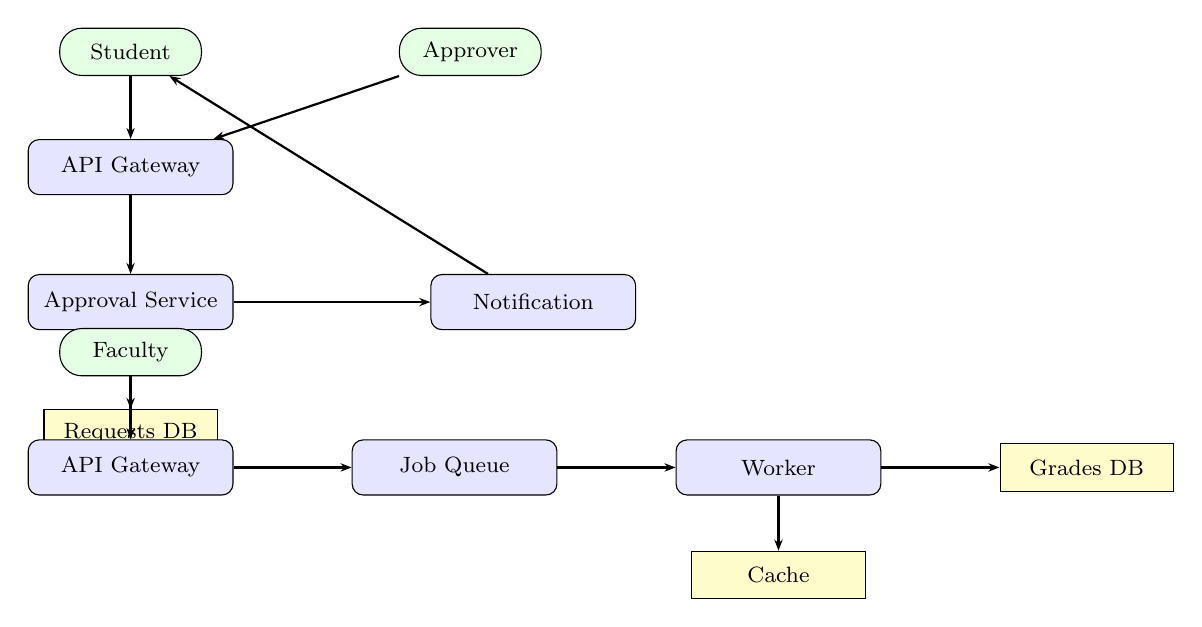
\begin{tikzpicture}[
  font=\footnotesize,
  node distance=1.0cm and 1.8cm,
  proc/.style={draw,rounded corners=4pt,fill=blue!10,minimum width=2.6cm,minimum height=0.7cm,align=center},
  store/.style={draw,fill=yellow!20,minimum width=2.2cm,minimum height=0.6cm,align=center},
  ext/.style={draw,fill=green!10,minimum width=1.8cm,minimum height=0.6cm,align=center,rounded corners=8pt},
  arrow/.style={-{Stealth[length=4pt]},thick},
]
\node[ext] (student) {Student};
\node[proc, below=0.8cm of student] (gw1) {API Gateway};
\node[proc, below=of gw1] (aps) {Approval Service};
\node[store, below=of aps] (rdb) {Requests DB};
\node[proc, right=2.5cm of aps] (notif) {Notification};
\node[ext, right=2.5cm of student] (approver) {Approver};

\draw[arrow] (student)  -- (gw1);
\draw[arrow] (gw1)      -- (aps);
\draw[arrow] (aps)      -- (rdb);
\draw[arrow] (approver) -- (gw1);
\draw[arrow] (aps)      -- (notif);
\draw[arrow] (notif)    -- (student);

\node[ext, below=3.2cm of student] (faculty) {Faculty};
\node[proc, below=0.8cm of faculty] (gw2) {API Gateway};
\node[proc, right=1.5cm of gw2] (queue) {Job Queue};
\node[proc, right=1.5cm of queue] (worker) {Worker};
\node[store, right=1.5cm of worker] (adb) {Grades DB};
\node[store, below=0.7cm of worker] (cachenode) {Cache};

\draw[arrow] (faculty) -- (gw2);
\draw[arrow] (gw2) -- (queue);
\draw[arrow] (queue) -- (worker);
\draw[arrow] (worker) -- (adb);
\draw[arrow] (worker) -- (cachenode);
\end{tikzpicture}
\caption{Data flow: outpass submission (top) and grade upload (bottom)}
\label{fig:dfd}
\end{figure}

\section{Async Processing Rationale}

Asynchronous processing is used for bulk uploads because: (1) HTTP timeout constraints (30--60 s) preclude synchronous processing of files with hundreds of records; (2) the job queue acts as a buffer against traffic spikes; (3) job state persisted in the database enables progress polling from any client instance without persistent WebSocket connections.

\section{Cache Architecture}

Grade data for student reads is served from a cache layer. The read-heavy, temporally stable nature of grade data makes caching effective:

\begin{equation}
  \text{Response latency} = \begin{cases} \sim 20\text{--}50\,\text{ms} & \text{cache hit} \\ \sim 100\text{--}300\,\text{ms} & \text{cache miss (DB query + cache write)} \end{cases}
\end{equation}

Cache entries are invalidated upon successful grade upload or bulk-update completion.

%%%% CHAPTER 9
\chapter{Database Design}

\section{Design Philosophy}

The UniZ database is designed around: (1) normalisation to at least 3NF; (2) UUID primary keys to prevent enumeration attacks; (3) audit fields (\field{createdAt}, \field{updatedAt}) on all mutable entities; (4) soft deletes via \field{isDeleted} flag.

\section{Core Entities}

\textbf{User:} \field{id} (UUID PK), \field{username} (unique), \field{passwordHash} (bcrypt), \field{role} (enum), \field{email} (unique).

\textbf{Student} extends User: \field{userId} (FK), \field{fullName}, \field{branch} (CSE/ECE/EEE/ME/CE), \field{year} (E1--E4), \field{is\_in\_campus} (boolean, default true), \field{gender} (M/F).

\textbf{Subject:} \field{id} (UUID PK), \field{code} (unique, e.g., \code{E2-SEM-1-CSE-3}), \field{name}, \field{credits}, \field{branch}, \field{year}, \field{semesterId}.

\textbf{GradeRecord:} \field{id} (UUID PK), \field{studentId} (FK), \field{subjectId} (FK), \field{semesterId}, \field{grade} (polymorphic). Unique constraint on (\field{studentId}, \field{subjectId}, \field{semesterId}).

\textbf{AttendanceRecord:} \field{id} (UUID PK), \field{studentId} (FK), \field{subjectId} (FK), \field{semesterId}, \field{attendedClasses}, \field{totalClasses}. Unique constraint on (\field{studentId}, \field{subjectId}, \field{semesterId}).

\textbf{OutpassRequest:} \field{id}, \field{studentId} (FK), \field{reason}, \field{fromDay}, \field{toDay}, \field{studentGender}, \field{currentLevel} (enum), \field{isApproved}, \field{isRejected}, \field{isExpired}, \field{requested\_time}, \field{comments} (JSON array).

\textbf{OutingRequest:} \field{id}, \field{studentId} (FK), \field{reason}, \field{fromTime}, \field{toTime}, \field{status} (pending/approved/rejected), \field{requested\_time}.

\textbf{UploadJob:} \field{id} (jobId), \field{type} (grades/attendance/students/publish), \field{status} (queued/processing/completed/failed), \field{percent}, \field{processed}, \field{total}, \field{errors} (JSON array), \field{createdBy} (FK).

\textbf{Banner:} \field{id}, \field{title}, \field{text}, \field{imageUrl} (nullable), \field{isPublished} (default false), \field{createdBy} (FK).

\section{Entity Relationship Diagram}

\begin{figure}[H]
\centering
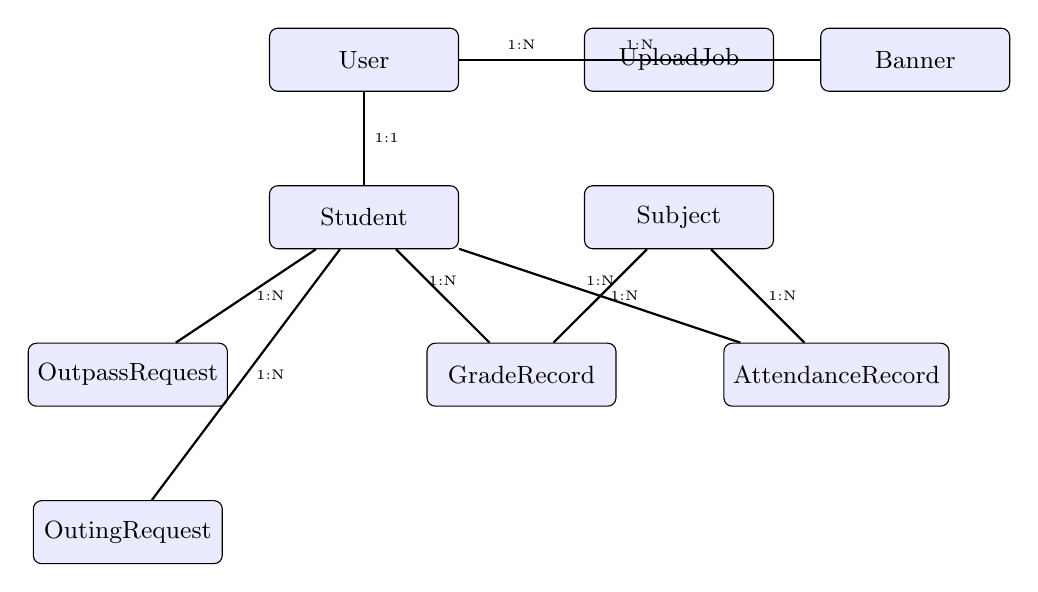
\begin{tikzpicture}[
  font=\small,
  entity/.style={draw,fill=blue!8,rounded corners=3pt,minimum width=2.4cm,minimum height=0.8cm,align=center},
  line/.style={thick},
]
\node[entity] (user)    at (0,0)   {User};
\node[entity] (student) at (0,-2)  {Student};
\node[entity] (subject) at (4,-2)  {Subject};
\node[entity] (grade)   at (2,-4)  {GradeRecord};
\node[entity] (att)     at (6,-4)  {AttendanceRecord};
\node[entity] (outpass) at (-3,-4) {OutpassRequest};
\node[entity] (outing)  at (-3,-6) {OutingRequest};
\node[entity] (job)     at (4,0)   {UploadJob};
\node[entity] (banner)  at (7,0)   {Banner};
\draw[line] (user)    -- node[midway,right]{\tiny 1:1} (student);
\draw[line] (student) -- node[midway,above]{\tiny 1:N} (grade);
\draw[line] (subject) -- node[midway,above]{\tiny 1:N} (grade);
\draw[line] (student) -- node[midway,right]{\tiny 1:N} (att);
\draw[line] (subject) -- node[midway,right]{\tiny 1:N} (att);
\draw[line] (student) -- node[midway,right]{\tiny 1:N} (outpass);
\draw[line] (student) -- node[midway,right]{\tiny 1:N} (outing);
\draw[line] (user)    -- node[midway,above]{\tiny 1:N} (job);
\draw[line] (user)    -- node[midway,above]{\tiny 1:N} (banner);
\end{tikzpicture}
\caption{Entity relationship diagram}
\label{fig:er}
\end{figure}

\section{Key Constraints}

\begin{table}[H]
\centering
\caption{Critical database constraints}
\label{tab:constraints}
\renewcommand{\arraystretch}{1.2}
\begin{tabularx}{\textwidth}{llX}
\toprule
\textbf{Entity} & \textbf{Type} & \textbf{Description} \\
\midrule
User & UNIQUE(username) & No two accounts share a username \\
User & UNIQUE(email) & No two accounts share an email \\
GradeRecord & UNIQUE(studentId, subjectId, semesterId) & One grade per student per subject per semester \\
AttendanceRecord & UNIQUE(studentId, subjectId, semesterId) & One attendance record per combination \\
OutpassRequest & CHECK(toDay $>$ fromDay) & Return must be after departure \\
OutingRequest & CHECK(sameDay(fromTime, toTime)) & Outing must be same-day \\
OutpassRequest & Partial unique index (active per student) & At most one non-terminal request per student \\
\bottomrule
\end{tabularx}
\end{table}

%%%% CHAPTER 10
\chapter{Security Architecture}

\section{JWT Authentication Lifecycle}

\subsection{Login and Token Issuance}
\begin{enumerate}[label=(\arabic*)]
  \item Client submits credentials to \api{POST /auth/login} over HTTPS.
  \item Server retrieves user record and verifies password against bcrypt hash using timing-safe comparison.
  \item On success, server constructs JWT payload: \field{sub} (username), \field{role}, \field{iat} (issued-at), \field{exp} (expiry).
  \item Server signs with HS256/RS256 and returns signed token.
\end{enumerate}

\subsection{Token Validation}
On every authenticated request, the API gateway: (1) extracts the Authorization header; (2) verifies JWT signature; (3) checks \field{exp} against current time (returns 401 if expired); (4) extracts \field{role} and evaluates RBAC decision.

\subsection{Session Invalidation}
Token invalidation is achieved through short expiry windows. Password changes via OTP recovery invalidate prior tokens by virtue of changed credentials.

\section{OTP Password Recovery}
\begin{enumerate}[label=(\arabic*)]
  \item User submits username to \api{POST /auth/otp}.
  \item Server generates six-digit cryptographically random OTP, stores it hashed with expiry timestamp.
  \item OTP delivered to registered institutional email.
  \item User submits OTP; server validates against stored hash and checks expiry.
  \item On valid OTP, user sets new password. OTP record is deleted (single-use).
\end{enumerate}

\section{Transport Security}
All communication occurs over HTTPS (TLS 1.2+). HTTP redirects to HTTPS at the reverse proxy. HSTS headers prevent protocol downgrade attacks.

\section{RBAC Enforcement}
RBAC middleware executes before route handlers, implementing a fail-closed design: routes without explicit role whitelist deny all access, preventing accidental exposure of undeclared endpoints. If the authenticated role is not in the route's whitelist, 403 Forbidden is returned before the handler executes.

\section{Input Validation and Injection Prevention}
All request bodies are validated against schema (required fields, types, ranges) before reaching service handlers. Database interactions use parameterised queries exclusively, eliminating SQL injection. File uploads are restricted by MIME type and extension server-side; uploaded files are never executed.

\section{Rate Limiting}
Submission endpoints are rate-limited per authenticated user using a sliding window algorithm. Requests exceeding the limit receive 429 with a Retry-After header.

%%%% CHAPTER 11
\chapter{Request Approval Engine}

\section{Finite State Machine Model}

The outpass approval engine is a deterministic finite-state machine over:

\begin{equation}
  \Sigma = \{\texttt{caretaker},\, \texttt{warden},\, \texttt{swo},\, \texttt{dean},\, \texttt{approved},\, \texttt{rejected}\}
\end{equation}

The transition function $\delta: \Sigma \times \text{Input} \to \Sigma$ is defined in Table~\ref{tab:statetrans}.

\begin{table}[H]
\centering
\caption{Outpass approval state transition table}
\label{tab:statetrans}
\renewcommand{\arraystretch}{1.3}
\begin{tabular}{llll}
\toprule
\textbf{Current State} & \textbf{Action} & \textbf{Actor Role} & \textbf{Next State} \\
\midrule
\code{caretaker} & approve & caretaker\_\{male$|$female\} & \code{warden} \\
\code{caretaker} & reject  & caretaker\_\{male$|$female\} & \code{rejected} \\
\code{warden}    & approve & warden\_\{male$|$female\}    & \code{swo} \\
\code{warden}    & reject  & warden\_\{male$|$female\}    & \code{rejected} \\
\code{swo}       & approve & swo                          & \code{dean} \\
\code{swo}       & reject  & swo                          & \code{rejected} \\
\code{dean}      & approve & dean                         & \code{approved} \\
\code{dean}      & reject  & dean                         & \code{rejected} \\
Any non-terminal & approve & director                     & \code{approved} \\
Any non-terminal & reject  & director                     & \code{rejected} \\
Any non-terminal & approve & dean                         & \code{approved} \\
\bottomrule
\end{tabular}
\end{table}

\subsection{State Machine Diagram}

\begin{figure}[H]
\centering
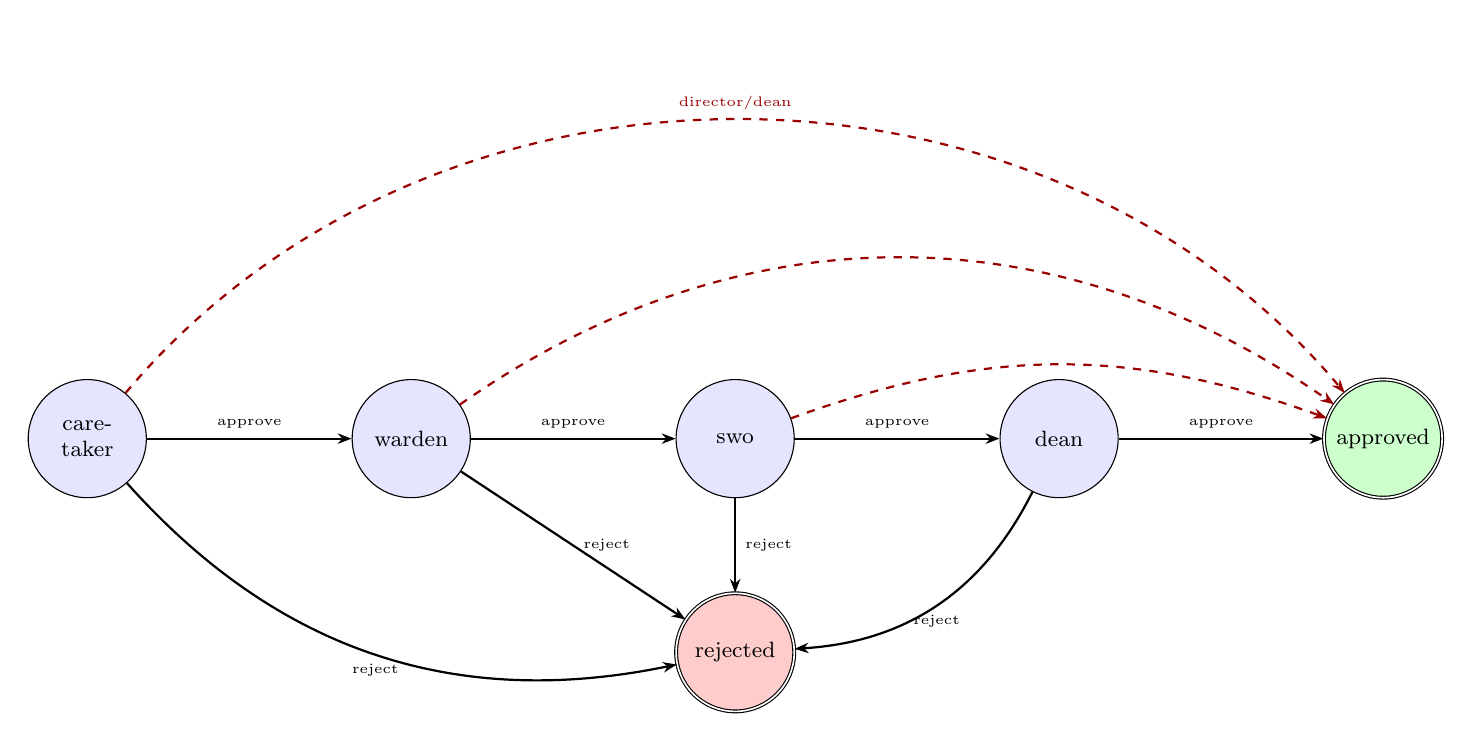
\begin{tikzpicture}[
  font=\small,
  node distance=2.6cm,
  state/.style={draw,circle,fill=blue!10,minimum size=1.5cm,align=center,font=\footnotesize},
  terminal/.style={draw,circle,fill=green!20,double,minimum size=1.5cm,align=center,font=\footnotesize},
  rejected/.style={draw,circle,fill=red!20,double,minimum size=1.5cm,align=center,font=\footnotesize},
  arrow/.style={-{Stealth[length=5pt]},thick},
]
\node[state]    (ct)  {care-\\taker};
\node[state]    (wd)  [right=of ct]  {warden};
\node[state]    (swo) [right=of wd]  {swo};
\node[state]    (dn)  [right=of swo] {dean};
\node[terminal] (ap)  [right=of dn]  {approved};
\node[rejected] (rj)  [below=1.2cm of swo] {rejected};
\draw[arrow] (ct) -- node[font=\tiny,above]{approve} (wd);
\draw[arrow] (wd) -- node[font=\tiny,above]{approve} (swo);
\draw[arrow] (swo) -- node[font=\tiny,above]{approve} (dn);
\draw[arrow] (dn) -- node[font=\tiny,above]{approve} (ap);
\draw[arrow] (ct) to[bend right=30] node[font=\tiny,below]{reject} (rj);
\draw[arrow] (wd) -- node[font=\tiny,right]{reject} (rj);
\draw[arrow] (swo) -- node[font=\tiny,right]{reject} (rj);
\draw[arrow] (dn) to[bend left=30] node[font=\tiny,below]{reject} (rj);
\draw[arrow,dashed,color=red!60!black] (ct) to[bend left=50] node[font=\tiny,above]{director/dean} (ap);
\draw[arrow,dashed,color=red!60!black] (wd) to[bend left=35] (ap);
\draw[arrow,dashed,color=red!60!black] (swo) to[bend left=20] (ap);
\end{tikzpicture}
\caption{Outpass approval state machine (dashed: director/dean override)}
\label{fig:statemachine}
\end{figure}

\section{Active Request Constraint}

The system enforces $|R_{\text{active}}(s)| \leq 1$ at both the application layer (pre-insert check) and database layer (partial unique index on \field{studentId} where status is non-terminal), providing defense in depth.

\section{Expiry Handling}

A background cron job identifies requests whose \field{fromDay} has elapsed while non-terminal. Such requests are transitioned to expired state (\field{isExpired}: \code{true}), retained for audit but excluded from the active queue and locked against further approval.

\section{Notification Triggers}

(1) \textbf{Rejection}: Any approver rejecting triggers immediate student email with rejection reason. (2) \textbf{Final approval}: Dean/director approval triggers student notification with approved window. Intermediate approvals do not notify students, reducing noise.

%%%% CHAPTER 12
\chapter{Performance and Optimisation}

\section{Grade Read Path Caching}

On first request, the service queries the database for grade records (a multi-join query). The result is stored in the cache under a student-ID-derived key. Subsequent reads bypass the database entirely. Cache entries are invalidated on grade upload completion or bulk-update. The \field{source} field in the response provides client-side observability.

\section{Batch Write Processing}

Bulk writes are processed in configurable batch sizes $B$. The number of database transactions is $\lceil N/B \rceil$ for $N$ records, amortising transaction overhead. Batch size is tuned to balance write throughput against lock contention.

\section{Dashboard Polling Strategy}

The security dashboard polls every 30 seconds with focus, falling back to every 5 minutes in the background. This reduces server load from idle background tabs while maintaining real-time responsiveness for active operators.

\section{Database Indexing}

Critical indexes: (1) OutpassRequest on (currentLevel, studentGender) for approval queue lookups; (2) OutpassRequest on studentId for constraint check and history; (3) GradeRecord on (studentId, semesterId) for student reads; (4) GradeRecord on (branch, year, semesterId) for batch queries; (5) Student on is\_in\_campus for outside-campus list.

\section{Pagination}

List endpoints implement page-based pagination. \field{limit} controls page size; \field{pagination} metadata carries page, totalPages, and total for client navigation.

%%%% CHAPTER 13
\chapter{Error Handling and Edge Cases}

\section{HTTP Error Response Convention}

All errors use a consistent envelope:
\begin{lstlisting}[caption={Standard error response},label={lst:error}]
{ "success": false, "error": "ERROR_CODE", "message": "Human-readable explanation" }
\end{lstlisting}

\begin{table}[H]
\centering
\caption{HTTP error codes in UniZ}
\label{tab:errors}
\renewcommand{\arraystretch}{1.2}
\begin{tabular}{cll}
\toprule
\textbf{Code} & \textbf{Meaning} & \textbf{Common Trigger} \\
\midrule
400 & Bad Request        & Missing fields, type errors, date ordering violations \\
401 & Unauthorized       & Missing, expired, or invalid JWT \\
403 & Forbidden          & Role not permitted for the resource/action \\
404 & Not Found          & Resource ID does not exist \\
409 & Conflict           & Active request constraint violated \\
429 & Too Many Requests  & Rate limit exceeded \\
500 & Internal Server Error & Unhandled server-side exception \\
\bottomrule
\end{tabular}
\end{table}

\section{Bulk Upload Error Handling}

Row-level errors are collected during worker processing and stored in the UploadJob \field{errors} array. A completed job may have both successful writes and row-level errors, enabling targeted correction without re-uploading the entire file.

\section{Expired Request Edge Cases}

A request that expires becomes irreversibly inert; a new request must be submitted. An approved request whose \field{toDay} has passed while the student is still outside creates a discrepancy; security staff must manually check-in via the API.

\section{Invalid Subject ID in Bulk Update}

The bulk-update endpoint silently skips records with unrecognised subject UUIDs, prioritising partial success. The \field{updated} count allows the caller to detect discrepancies.

%%%% CHAPTER 14
\chapter{Discussion}

\section{Client-Side Role Filtering Design}

Returning all outpass records from a single endpoint without server-side role filtering provides API simplicity and audit flexibility. For large institutions with hundreds of concurrent requests, server-side filtering or pagination should be introduced to manage payload size.

\section{Forward as Approve Alias}

The forward action is semantically identical to approve at the backend. This preserves a useful UX distinction without introducing state complexity. As the platform matures, forward could be distinguished in analytics (e.g., not counting as an explicit approval for caretaker performance metrics).

\section{Sync vs. Async Upload}

Synchronous processing would be simpler but would fail under HTTP timeout constraints for large cohorts. The async pipeline introduces operational complexity (job monitoring, error collection, cache invalidation sequencing) but provides a robust foundation for arbitrarily large uploads.

\section{Active Request Constraint Design}

The $|R_{\text{active}}| \leq 1$ constraint prevents gaming the approval system (submitting multiple concurrent requests to increase approval probability). The defense-in-depth implementation at both application and database layers ensures the constraint holds even under concurrent submissions.

\section{Limitations and Future Work}

\begin{enumerate}[label=(\arabic*)]
  \item \textbf{Push notifications:} Integration with Web Push API would enable real-time in-app notifications, reducing reliance on email delivery.
  \item \textbf{Biometric gate verification:} Integration with hardware biometric readers at gates would eliminate manual ID entry and reduce proxy exit risk.
  \item \textbf{Analytics dashboard:} Approval rate trends, average processing time per level, and attendance distribution across branches would provide institutional insight.
  \item \textbf{Multi-campus support:} A multi-tenant extension partitioned by campus identifier would enable other RGUKT campuses to share the platform.
  \item \textbf{WebSocket real-time updates:} Replacing polling with WebSocket push would reduce unnecessary HTTP traffic for upload progress and security dashboards.
\end{enumerate}

%%%% CHAPTER 15
\chapter{Conclusion}

This report has presented UniZ, a production-deployed distributed university administration platform for RGUKT Ongole. UniZ addresses a concrete operational problem: the fragmentation of campus management across paper-based workflows, disconnected spreadsheets, and ad hoc communication channels.

The platform is engineered around three foundational abstractions. First, a \textbf{formal RBAC model} with eleven distinct roles strictly enforced at the API gateway ensures each user operates within precisely the capability surface appropriate to their institutional function. Second, a \textbf{deterministic approval state machine} with six states, well-defined transition semantics, override logic for high-authority roles, and automatic expiry handling provides reliable, auditable campus mobility governance. The active-request constraint enforced at both application and database layers provides defense in depth. Third, an \textbf{asynchronous academic data pipeline} decouples bulk data ingestion from record processing, enabling grade and attendance management at cohort scale while serving student reads from a cache layer with sub-50\,ms latency.

The platform is deployed as a Progressive Web Application, delivering a high-quality installable experience across iOS, Android, and desktop without app store distribution. Security is enforced through JWT-based stateless authentication, OTP-based password recovery, parameterised database queries, and HTTPS-only transport.

UniZ demonstrates that carefully designed software systems can substantially improve administrative efficiency in residential educational institutions. The lessons learned -- treating approval workflows as formal state machines, role immutability as a security primitive, and async processing as a scalability necessity -- are broadly applicable to institutional administration platforms beyond the university domain.

% ─── References ───────────────────────────────────────────────────────────────
\chapter*{References}
\addcontentsline{toc}{chapter}{References}

\begin{enumerate}[label={[\arabic*]}]
  \item R. Sandhu, E. Coyne, H. Feinstein, and C. Youman, ``Role-Based Access Control Models,'' \textit{IEEE Computer}, vol.~29, no.~2, pp.~38--47, Feb. 1996.
  \item R. Fielding, ``Architectural Styles and the Design of Network-based Software Architectures,'' Ph.D. dissertation, Univ. of California, Irvine, 2000.
  \item M. Jones, J. Bradley, and N. Sakimura, ``JSON Web Token (JWT),'' IETF RFC~7519, May 2015.
  \item A. Russell, ``Progressive Web Apps: Escaping Tabs Without Losing Our Soul,'' \textit{Infrequently Noted}, Jun. 2015.
  \item E. Gamma, R. Helm, R. Johnson, and J. Vlissides, \textit{Design Patterns: Elements of Reusable Object-Oriented Software}. Addison-Wesley, 1994.
  \item M. Fowler, \textit{Patterns of Enterprise Application Architecture}. Addison-Wesley, 2002.
  \item C. J. Date, \textit{An Introduction to Database Systems}, 8th ed. Addison-Wesley, 2003.
  \item Open Web Application Security Project (OWASP), ``OWASP Top Ten,'' 2021. [Online]. Available: \url{https://owasp.org/www-project-top-ten/}
  \item National Institute of Standards and Technology, ``Guide to Attribute Based Access Control (ABAC),'' NIST SP 800-162, Jan. 2014.
  \item T. Berners-Lee, R. Fielding, and L. Masinter, ``Uniform Resource Identifier (URI): Generic Syntax,'' IETF RFC~3986, Jan. 2005.
  \item D. Barroso and U. Hoelzle, \textit{The Datacenter as a Computer}, 2nd ed. Morgan \& Claypool, 2013.
  \item M. T. Goodrich and R. Tamassia, \textit{Introduction to Computer Security}. Pearson, 2011.
\end{enumerate}

% ─── Appendices ───────────────────────────────────────────────────────────────
\appendix

\chapter{Complete API Endpoint Reference}

\begin{longtable}{p{4.3cm}p{1.6cm}p{3.2cm}p{3.5cm}}
\caption{UniZ complete API endpoint reference}\label{tab:apiref}\\
\toprule
\textbf{Endpoint} & \textbf{Method} & \textbf{Role Access} & \textbf{Description} \\
\midrule
\endfirsthead
\multicolumn{4}{c}{Table \thetable{} -- continued}\\
\toprule
\textbf{Endpoint} & \textbf{Method} & \textbf{Role Access} & \textbf{Description} \\
\midrule
\endhead
\midrule\multicolumn{4}{r}{Continued on next page}\\
\endfoot
\bottomrule
\endlastfoot
/auth/login & POST & All & Credential authentication \\
/auth/otp & POST & All (unauth) & OTP password recovery \\
/system/health & GET & Public & Service health check \\
/academics/grades & GET & Student & Own grade records \\
/academics/grades/batch & GET & Dean, Director, Webmaster & Batch grade query \\
/academics/grades/add & POST & Faculty, Admin & Add single grade \\
/academics/grades/bulk-update & PUT & Dean, Webmaster & Bulk grade correction \\
/academics/grades/template & GET & Faculty, Admin & Download grade template \\
/academics/grades/upload & POST & Faculty, Admin & Bulk grade upload \\
/academics/grades/upload/progress & GET & Faculty, Admin & Upload job progress \\
/academics/grades/publish-email & POST & Director & Publish results via email \\
/academics/grades/publish/progress & GET & Director & Publish job progress \\
/academics/grades/download/:semId & GET & Admin & Download grade report \\
/academics/attendance & GET & Student & Own attendance records \\
/academics/attendance/add & POST & Faculty & Add single attendance \\
/academics/attendance/template & GET & Faculty, Admin & Download attendance template \\
/academics/attendance/upload & POST & Faculty, Admin & Bulk attendance upload \\
/academics/attendance/upload/progress & GET & Faculty, Admin & Upload job progress \\
/academics/attendance/download/:semId & GET & Admin & Download attendance report \\
/academics/attendance/publish-email & POST & Director & Publish attendance email (deprecated) \\
/requests/outpass & POST & Student & Submit outpass \\
/requests/outpass/all & GET & Caretaker, Warden, SWO, Dean, Director, Security & All outpass records \\
/requests/outing & POST & Student & Submit outing \\
/requests/outing/all & GET & Security, Director, Admin & All outing records \\
/requests/history & GET & Student & Own request history \\
/requests/outside & GET & Admin, Security, Director & Currently outside students \\
/requests/:id/approve & POST & Caretaker, Warden, SWO, Dean, Director & Approve request \\
/requests/:id/reject & POST & Caretaker, Warden, SWO, Dean, Director & Reject request \\
/requests/:id/forward & POST & Caretaker, Warden, SWO, Dean, Director & Forward request \\
/requests/:id/checkout & POST & Security, Director & Gate check-out \\
/requests/:id/checkin & POST & Security, Director & Gate check-in \\
/requests/security/summary & GET & Security & Dashboard metrics \\
/profile/student/search & POST & Dean, Director, Security & Student search \\
/profile/student/status & PUT & Director, Security & Manual status override \\
/profile/admin/banners & GET & Admin roles & List banners \\
/profile/admin/banners & POST & Webmaster & Create banner \\
/profile/admin/banners/:id/publish & POST & Webmaster & Publish/unpublish banner \\
/admin/student/template & GET & Admin & Download student template \\
/admin/student/upload & POST & Admin & Bulk student upload \\
\end{longtable}

\chapter{Approval Workflow Sample Sequence}

\textbf{Step 1 -- Student submits outpass:}
\begin{lstlisting}[caption={Outpass submission and initial response},label={lst:app1}]
POST /api/v1/requests/outpass
Authorization: Bearer <student_token>
{
  "reason": "Home visit for Diwali festival",
  "fromDay": "2026-11-01T09:00:00Z",
  "toDay":   "2026-11-05T18:00:00Z",
  "studentGender": "M"
}
Response 200:
{ "success": true, "data": { "id": "req-789",
  "currentLevel": "caretaker", "isApproved": false,
  "createdAt": "2026-10-28T10:00:00Z" } }
\end{lstlisting}

\textbf{Step 2 -- Caretaker approves:}
\begin{lstlisting}[caption={Caretaker approval},label={lst:app2}]
POST /api/v1/requests/req-789/approve
Authorization: Bearer <caretaker_token>
{ "comment": "Parents verified via phone call" }
Response 200:
{ "success": true, "msg": "Request approved and forwarded to next level." }
\end{lstlisting}

\textbf{Step 3 -- Director grants final approval (override):}
\begin{lstlisting}[caption={Director final approval},label={lst:app3}]
POST /api/v1/requests/req-789/approve
Authorization: Bearer <director_token>
{ "comment": "Approved." }
Response 200:
{ "success": true, "msg": "Request approved and forwarded to next level." }
\end{lstlisting}
After Step 3: \code{isApproved: true}; student notified; security can verify at gate.

\chapter{RBAC Formal Specification}

Let $U$ be the set of all users, $R$ the set of roles (as defined in Chapter~3), $O$ the set of protected resources, $A$ the set of actions (\{read, write, approve, reject, override, publish, manage\}), and $P \subseteq R \times O \times A$ the permission relation. The role assignment $\text{assign}: U \to R$ is a total function (every user has exactly one role).

\vspace{0.3cm}
The access decision:
\begin{equation}
  \text{permit}(u, o, a) = \exists\, (r, o', a') \in P \text{ s.t. } r = \text{assign}(u) \land o' = o \land a' = a
\end{equation}

Role immutability:
\begin{equation}
  \forall\, u \in U,\, \forall\, t_1 < t_2:\, \text{assign}_{t_1}(u) = \text{assign}_{t_2}(u)
\end{equation}

Gender-partitioned role constraint:
\begin{equation}
  \text{permit}(u, \text{req}, \text{approve}) \implies \text{assign}(u) \in \{\text{caretaker\_male, caretaker\_female}\} \Rightarrow \text{req.gender} = \text{gender}(\text{assign}(u))
\end{equation}

Active-request invariant:
\begin{equation}
  |R_{\text{active}}(s)| = |\{ r \in \text{Requests}(s) \mid r.\text{currentLevel} \notin \{\texttt{approved}, \texttt{rejected}, \texttt{expired}\}\}| \leq 1
\end{equation}

\end{document}
